\chapter{Implementacja algorytmu}

Problem układania planu zajęć można próbować rozwiązać za pomocą algorytmu przeszukiwania z tabu (ang. \textit{Tabu search}). Jednak implementacjia tego algorytmu jest trudna, z uwagi na dużą złożoność problemu układania planu zajęć. Rozmiar generowanego sąsiedztwa lub stopień złożoności funkcji oceny, to tylko niektóre z nich. Poniżej omówiona została implementacjia algorytmu przeszukiwania z tabu oraz jej specyfikacja wewnętrzna i zewnętrzna.

\section{Implementacja}

Implementacja algorytmu została napisana w języku C\#. Język ten został wybrany z uwagi na dużą liczbę bezpłatnych bibliotek oraz możliwość dostępu do bardzo dobrej dokumentacji technicznej. Nie bez znaczenia był także fakt dużej popularności języka, co skutkuje większymi możliwościami uzyskania pomocy na forach programistycznych.

\subsection{Wprowadzanie danych}

Pierwszym problemem, który stanął przed autorem tej pracy, było wprowadz danych, korzystając z formatu XHSTT. Format ten został omówiony w poprzednim rozdziale. Ponieważ dane zawarte w tym formacie zapisane są w języku XML, skorzystano z biblioteki systemowej  \textit{Xml.Linq}, która pozwala traktować dokument XML jako bazę danych i wysyłać do niej stosowne zapytania. Przykład wprowadzania instancji problemu układania planu zajęć za pomocą tej biblioteki przedstawiony został na rysunku 5.1. Biblioteka \textit{Xml.Linq} stanowiła spore ułatwienie, jednak w dalszym ciągu trudności sprawiał złożony charakter dokumentu, ponieważ każde zagnieżdżenie musiało być wczytane za pomocą odpowiedniego wiersza kodu. 

\begin{figure}
	\centering
	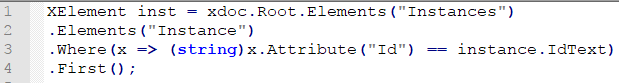
\includegraphics {linqprzyklad}
	\caption{Przykład wprowadzania instancji problemu układania planu zajęć za pomocą biblioteki \textit{Xml.Linq}.}
	\label{fig: linqprzyklad}
\end{figure}

Wprowadzone dane zapisywane są w bazie danych, dlatego każde kolejne wykonanie aplikacji umożliwia pracę na już wczytanych danych. Jak stwierdzono w poprzednich rozdziałach, założono, że wprowadzone dane zawierają zdarzenia z przypisanymi wcześniej zasobami, takimi jak nauczyciel, sala i grupa.

\subsection{Generowanie rozwiązania początkowego}

Algorytm przeszukiwania z tabu w celu znalezienia najlepszego rozwiązania musi rozpocząć się od pewnego rozwiązania początkowego. Warto przypomnieć, że algorytm przeszukiwania z tabu jest algorytmem heurystycznym. W zależności od tego,z jakim rozwiązaniem początkowym rozpocznie on swoje działanie, może uzyskać różne rezultaty po określonej liczbie iteracji. Stworzenie początkowego planu zajęć, w którym wszystkie zajęcia rozpoczynałyby się np. w poniedziałek, w pierwszym dostępnym oknie czasowym, mogłoby spowodować znaczne wydłużenie czasu,pow którym algorytm znajdzie dostatecznie dobre rozwiązanie. Wydłużony czas wynikał by z niskiej oceny takiego planu i dłuższej ,,drogi'', jaką algorytm musi pokonać, by dojść do dobrego rozwiązania. Zdecydowano się więc na wprowadzenie elementu probabilistycznego, by zróżnicować początkowy plan zajęć. Każdemu wydarzeniu przypisywane jest losowe okno czasowe. Dobrym pomysłem byłoby zastosowanie algorytmu, który utworzył by początkowy plan zajęć z jeszcze lepszą oceną. Jednak, z uwagi na ograniczony czas implementacji, zdecydowano się pozostać przy rozwiązaniu losowym.

\subsection{Generowanie dostępnych ruchów algorytmu}

By ułatwić generowanie sąsiedztwa niezbędnego w dalszym działaniu algorytmu, zdecydowano się na generowanie wszystkich dostępnych ruchów dla danego kroku algorytmu. Przez ruch rozumiana jest para: wydarzenie i okno czasowe. Oznacza to, że wybranemu wydarzeniu przyporządkowane zostaje określone okno czasowe. Generowane są więc wszystkie pary, których liczba równa jest liczbie wydarzeń pomnożonej przez liczbę okien czasowych. Tak zdefiniowany ruch, może być w łatwy sposób wykorzystany podczas generacji sąsiedztwa bieżącego rozwiązania (tj. planu zajęć). Co więcej, tak wygenerowane pary nie są zależne od aktualnego rozwiązania, i dla każdego kroku algorytmu są zawsze takie same (o ile nie znajdują się na liście tabu). Dzięki temu, można łatwo reprezentować ruch jako parę indeksów i przechowywać go na liście tabu. Liczba wszystkich dostępnych ruchów określa rozmiar sąsiedztwa, które algorytm powinien przeszukać w danym kroku. Ponieważ liczba ta jest duża, konieczne było ograniczenie przeszukiwanego sąsiedztwa.

\subsection{Generowanie i ocenianie sąsiedztwa dla wybranego rozwiązania}

W ramach jednej iteracji, algorytm powinien wygenerować sąsiedztwo dla bierzącego rozwiązania, ocenić każdego sąsiada i wybrać najlepszego z nich. Ponieważ obliczenie funkcji oceny rozwiązania jest bardzo kosztowne, konieczne było ograniczenie rozmiaru przeszukiwanego sąsiedztwa. Rozmiar ten jest jednym z parametrów algorytmu. Po raz kolejny zdecydowano się wprowadzić element probabilistyczny. Z puli dostępnych ruchów wybierane są ruchy w sposób losowy. Każdy z wylosowanych ruchów wykonywany jest dla aktualnego rozwiązania, tworząc nowe rozwiązanie, wchodzące w skład sąsiedztwa rozwiązania aktualnego. Tak wygenerowane sąsiedztwo jest oceniane i wybierane jest rozwiązanie najlepsze spośród dostępnych rozwiązań. Ruch, który doprowadził nas do rozwiązania najlepszego trafia na listę tabu. Następnie wybrane rozwiązanie porównywane jest z rozwiązaniem globalnie najlepszym, jakie do tej pory udało się znaleźć. Jeżeli nowe rozwiązanie jest lepsze, to staje się rozwiązaniem najlepszym globalnie. Ostatnim krokiem w ramach jednej iteracji algorytmu jest aktualizowanie listy Tabu. Dla każdego elementu aktualizowany jest czas jego trwania na liście tabu. Jeżeli jest on równy zeru, to ruch trafia z powrotem do zbioru dostępnych ruchów algorytmu.

\subsection{Funkcja oceny rozwiązania}

Najtrudniejszym elementem implementacji była funkcja oceny rozwiązania (tj. planu zajęć). Z uwagi na konieczność sprawdzania wielu warunków w stosunku do wielu elementów, jest to najbardziej czasochłonna część wykonania algorytmu. Wszystkie ograniczenia, które ma spełniać otrzymany plan zajęć muszą być badane w tej funkcji. Funkcja ta decyduje o jakości otrzymanego planu i daje duże możliwości, by w przyszłości ją udoskonalić.

Zdecydowano się wybrać do implementacji następujące ograniczenia:
\begin{itemize}
\item przypisanie wszystkim zdarzeniom określonego czasu,
\item unikanie konfliktów między zasobami,
\item unikanie dzielenia zajęć trwających dłużej niż jedno okno czasowe,
\item minimalizacja pustych okien czasowych między zdarzeniami dla grup uczniów.
\end{itemize} Każde z tych ograniczeń ma przyporządkowaną określoną wartość kary, która jest dodawana do końcowej oceny rozwiązania za każdym razem, gdy ograniczenie nie jest spełnione.

Każde zdarzenie musi mieć przypisane okno czasowe. Podczas oceny tego ograniczenia, sprawdzane są wszystkie wydarzenia. Za każdym razem, gdy któreś z wydarzeń nie będzie miało przypisanego okna czasowego, nałożona zostanie odpowiednia kara. Ograniczenie to miało zastosowanie tylko w początkowej fazie implementacji algorytmu, kiedy istaniała konieczność sprawdzania poprawności wykonania algorytmu. W dalszej fazie implementacji zdecydowano, że każde zdarzenie już podczas generacji rozwiązania początkowego ma przypisane okno czasowe, a nie ma możliwości, by algorytm usunął przypisane okno czasowe. Jedynymi zmianami może być przypisanie nowego okna czasowego. Z tego powodu ograniczenie to zostało pominięte.

Ograniczenie związane z unikaniem konfliktów między zasobami sprawdzane jest w następujący sposób. Dla każdego okna czasowego wyszukiwane są wszystkie zdarzenia, które w nim występują. Konieczne jest również przeszukanie dwóch okien czasowych w tył, by sprawdzić czy nie ma tam zajęć o długości dwóch lub trzech jednostek czasu. Po znalezieniu wszystkich zdarzeń, przeszukiwane są wszystkie zasoby do nich przypisane. Każdy zasób sprawdzany jest pod kątem wystąpienia po raz kolejny w tym samym oknie czasowym. Za każde dodatkowe wystąpnie zasobu nakładana jest stosowna kara. Sprawdzanie tego ograniczenia ma największą złożoność obliczeniową, ponieważ wymaga ono wielokrotnego sprawdzania zasobów.

Ograniczenie dotyczące unikania dzielenia zajęć trwających dłużej niż jedno okno czasowe może być złamane np. w przypadku, gdy zajęcia o czasie trwania dwóch okien czasowych, przypisane są na ostatnie okno czasowe danego dnia. Wtedy druga godzina zajęć przypisana jest w pierwszym oknie czasowym dnia następnego. Oczywiście nie jest to pożądane. By wykryć złamanie tego ograniczenia konieczne jest sprawdzenie wszystkich zajęć o czasie trwania dłuższym niż jedno okno czasowe. Dla każdego z tych zajęć sprawdzane są kolejne okna czasowe występujące po nim (w zależności od długości zajęć jest to jedno lub dwa okna czasowe). Jeżeli okna czasowe przypadające na jedno zajęcie należą do różnych dni, to nakładana jest ustalona kara.

Wszystkie wyżej wymienione ograniczenia można było określić jako ograniczenia twarde. Kara za ich złamanie jest bardzo wysoka. Ostatnie ograniczenie jest ograniczeniem miękkim. Kara za jego złamanie to około 10\% wartości kary poprzednich ograniczeń. Minimalizacja pustych okien czasowych między zdarzeniami dla grup uczniów nie jest obowiązkowa aby plan był poprawny. Brak tych okien jest jednak pożądany przez uczniów. By sprawdzić to ograniczenie konieczne jest przeszukanie planu dla każdej klasy z osobna. Jeżeli dla danej klasy, w danym dniu, wystąpiły już zajęcia, a następnie wystąpiło puste okno czasowe, a po nim kolejne zajęcia, to nałożona zostanie kara. Kara jest zależna od liczby pustych okien czasowych między zajęciami.

\section{Specyfikacja wewnętrzna programu}

Poprzedni podrozdział miał na celu przedstawienie pomysłu i sposobu w jaki zaimplementowany został algorytm przeszukiwania z tabu. Ten podrozdział zawiera szczegóły techniczne implementacji, opis użytych narzędzi, używanych klas oraz zawiera najistotniejsze fragmenty kodu.

\subsection{Użyte narzędzia}

Podczas implementowania algorytmu przeszukiwania z tabu użyto następujących narzędzi:

\begin{itemize}
	\item Język programowania C\# - jest to obiektowy język programowania, którego początki sięgają roku 1998. Został zaprojektowany dla firmy Microsoft przez Andersa Hejlsberga. Program napisany w tym języku jest kompilowany do języka \textit{Common Intermediate Language} (CIL), który jest wykonywany w środowisku \textit{.NET Framework}. Jest to język prosty, o dużych możliwościach i wielu cechach wspólnych z językami programowania C++ oraz Java \cite{Csharp}. 
	
	\item Biblioteka Linq - Language-Integrated Query (LINQ) pozwala odczytywać dane pochodzące z różnych źródeł w postaci obiektów. Biblioteka udostępnia funkcje filtrujące i wyszukujące, które odpowiednio użyte w znacznej mierze przyspieszają działanie programu. W implementacji algorytmu, którego dotyczy praca, zapytania Linq ułatwiają komunikację z bazą danych oraz czytanie dokumentów XML.
	
	\item Windows Forms - interfejs programowania graficznych aplikacji należący do środowiska \textit{.NET Framework}. Służy do tworzenia aplikacji z graficznym interfejsem użytkownika, umożliwiająca obsługę zdarzeń napływających od użytkownika. Obecnie interfejs wypierany jest przez interfejs Windows Presentation Foundation  (\textit{WPF}). Jednak mimo tego, dzięki swej prostocie i przejrzystości, jest dalej używany przez programistów.
	 
	\item Entity Framework - jest to bezpłatne oprogramowanie typu Object Relational Mapping (ORM), pozwalające odwzorować relacyjną bazę danych za pomocą architektury obiektowej. Dzięki temu narzędziu programista może w łatwy sposób zaprojektować bazę danych nie mając wiedzy na temat języka SQL. Stosując podejście \textit{code first} można zaprojektować tylko klasy bazowe, a resztę powierzyć narzędziu Entity Framework, które utworzy odpowiednią strukturę bazy danych.
	 
	\item Microsoft Visual Studio 2015 - zintegrowane środowisko programistyczne firmy Microsoft, umożliwiające pisanie i kompilowanie aplikacji w językach takich jak C\#, C++, C czy Visual Basic, na różne platformy. Dzięki dużej liczbie narzędzi umożliwia łatwe testowanie i debagowanie kodu, oraz pozwala szybko tworzyć nowe aplikacje. Jest to naturalny wybór dla języka programowania C\#.
	
	\item SQL Server 2014 Managment Studio - zintegrowane środowisko do zarządzania bazami danych. Zawiera narzędzia do konfigurowania i monitorowania baz danych. Umożliwia budowę zapytań i oglądanie tabel w bazie danych. Autor pracy wykorzystał to środowisko do testowania poprawności wykonanych operacji i analizy uzyskanych wyników.
\end{itemize}

\subsection{Opis klas i ważniejszych funkcji}

Aplikacja zapisana jest w kilku folderach. Każdy z folderów zawiera klasy realizujące odrębne funkcje aplikacji. Folder \textit{Code} zawiera klasy realizujące algorytm wyszukiwania.  W folderze \textit{Data} znajdują się klasy służące do translacji plików wejściowych XML na obiekty, i zapisywania nowo powstałych obiektów do bazy danych. Folder \textit{Model} zawiera klasy odwzorowujące obiekty znajdujące się w bazie danych. Znajdują się więc tu klasy takie jak \textit{Instance, Event, Resource}. Ostatni folder, \textit{ViewModel}, przechowuje klasy realizujące przygotowanie danych to zaprezentowania ich w interfejsie graficznym. Poza folderami znajduje się osobna klasa \textit{Form1}, która obsługuje interfejs graficzny użytkownika.

Poniżej przedstawiono ważniejsze klasy programu wraz z opisem funkcji w nich zawartych.

\begin{itemize}
	\item  \textit{Code/SolutionManager} - klasa zawiera szkielet algorytmu przeszukiwania z tabu. Jest to główna klasa algorytmu.  Znajdują się w niej funkcja rozwiązująca problem układania planu zajęć dla instancji o podanym identyfikatorze. Klasa ta zawiera również funkcje zapisującą raport działania algorytmu do pliku txt oraz funkcję wyświetlającą rozwiązanie na konsolę. Główna funkcja klasy zaprezentowana została na rysunku 5.2.
	
	\begin{figure}
	\centering
	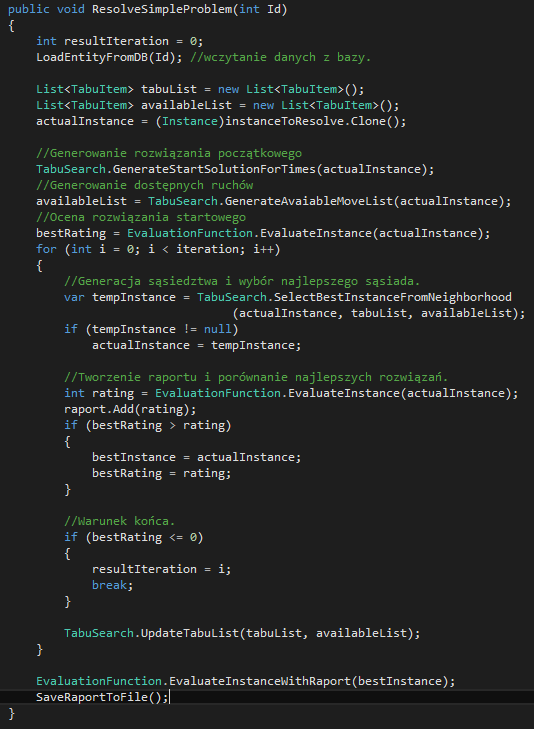
\includegraphics {ResolveSimpleProblem}
	\caption{Funkcja \textit{ResolveSimpleProblem} zawierająca szkielet algorytmu Tabu search. }
	\label{fig: ResolveSimpleProblem}
	\end{figure}

	\item \textit{Code/TabuSearch} - klasa zawieraja statyczne funkcje służące do rozwiązywania problemu za pomocą algorytmu przeszukiwania z tabu. Znajdują się tu funkcję generujące dostępne ruchy, losowe rozwiązanie startowe, aktualizujące listę tabu, generujące sąsiedztwo i wybierające z nich najlepszego osobnika. W tej klasie znajdują się najważniejsze fragmenty kodu implementujące algorytm przeszukiwania z tabu. Funkcja generująca sąsiedztwo i wybierająca z niego najlepszą instancje została zaprezentowana na rysunku 5.3.

	\begin{figure}
	\centering
	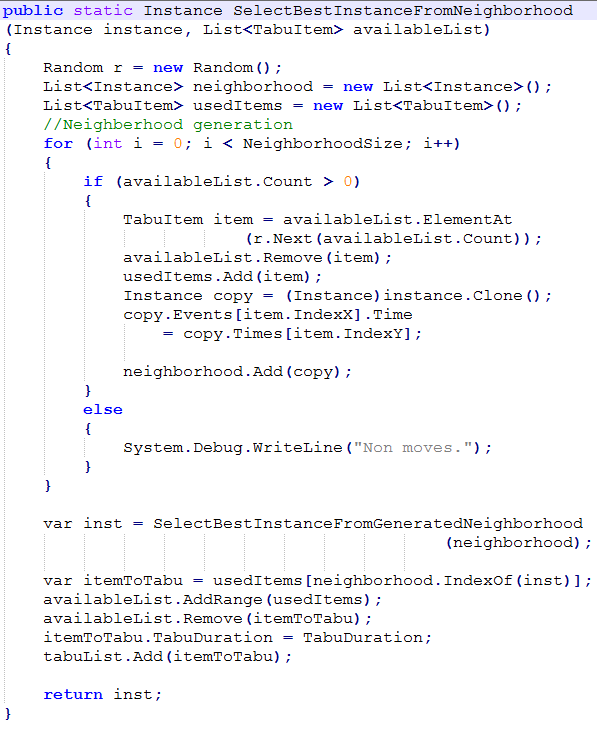
\includegraphics {SelectbestInstance}
	\caption{Funkcja \textit{SelectBestInstanceFromNeighborhood} generująca sąsiedztwo i wybierająca najlepszego sąsiada. }
	\label{fig: SelectbestInstance}
	\end{figure}

	\item \textit{Code/EvaluationFunction} -  w skład tej klasy wchodzą funkcje oceniające bieżące rozwiązanie uzyskane przez algorytm. Znajduje się tu implementacja wszystkich ograniczeń, jakie mają być uwzględnione w rozwiązaniu. Klasę tę można w łatwy sposób rozszerzyć dodając kolejne funkcje oceniające, które odpowiadają kolejnym ograniczeniom.
	 
	\item \textit{Code/TabuItem} - klasa reprezentująca pojedynczy ruch w algorytmie przeszukiwania z tabu. Jako ruch rozumiana jest para dwóch indeksów, pierwszy z nich odpowiada identyfikatorowi zdarzenia, a drugi to identyfikator okna czasowego, które w danym ruchu jest do tego zdarzenia przypisane.  Elementy klasy przechowywane są na liście tabu, dlatego klasa zawiera dodatkową właściwość, jaką jest czas trwania na liście tabu dla danego elementu.
	 
	\item  \textit{Data/XMLLoader} - w tej klasie zawarte są funkcje przekształcające dane wejściowe w formacie XHSTT, zapisane w języku XML, na klasy modelu. Znajduje się tu również funkcja zapisująca odczytaną instancje do bazy danych.
	
	\item \textit{Form1} - klasa obsługująca interfejs użytkownika. Zawiera funkcje reagujące na każdą wykonaną przez użytkownika czynność oraz funkcje wypisujące dane do odpowiednich obiektów interfejsu.
\end{itemize}

\section{Specyfikacja zewnętrzna}

	Po zainicjowaniu działania aplikacji wyświetlane jest okno główne przedstawione na rysunku 5.4. Przy pierwszym wykonaniu aplikacji użytkownik powinien wczytać instancje z pliku wejściowego. Może to wykonać za pomocą przycisku ,,Load instance from file'', który znajduje się w prawym górnym rogu okna. Otworzy się okno dialogowe, gdzie należy wskazać plik XML zawierający dane wejściowe dla problemu rozwiązywania planu zajęć, zapisane w formacie XHSTT. Po wczytaniu wielu instancji (lub po ponownym zainicjowaniu działania aplikacji), użytkownik może wybrać instancje do rozwiązania. Służy do tego rozwijana lista w lewym górnym rogu okna.
	
	Przycisk ,,Resolve'' służy do wykonania algorytmu. Działanie algorytmu jest monitorowane, a postępy wyświetlane są na konsoli na dole okna aplikacji. Po zakończeniu obliczeń, ułożony plan zajęć można oglądać w tabeli. Rozwijana lista nad tabelą służy do wyboru klasy, dla której ma zostać zaprezentowany plan zajęć.
	
	Użytkownik może zmieniać parametry algorytmu. Algorytm ma trzy parametry, których opis znajduje się poniżej:
	
	\begin{itemize}
		\item Iterations - maksymalna liczba iteracji jaką algorytm wykona w czasie rozwiązywania problemu układania planu zajęć. Jeżeli algorytm wcześniej znajdzie rozwiązanie, na które nie jest nałożona żadna kara, to zakończy swoje działanie.
		\item Tabu duration - parametr oznaczający czas pozostawania pojedynczego ruchu na liście tabu. Długość mierzona jest liczbą iteracji algorytmu.
		\item Neighborhood - rozmiar sąsiedztwa jakie zostanie losowo wybrane i przeszukane podczas jednej iteracji algorytmu. Rozmiar sąsiedztwa nie powinien być większy od liczby wszystkich dostępnych ruchów, które może wykonać algorytm (pełne sąsiedztwo).
	\end{itemize}
	
	\begin{figure}
	\centering
	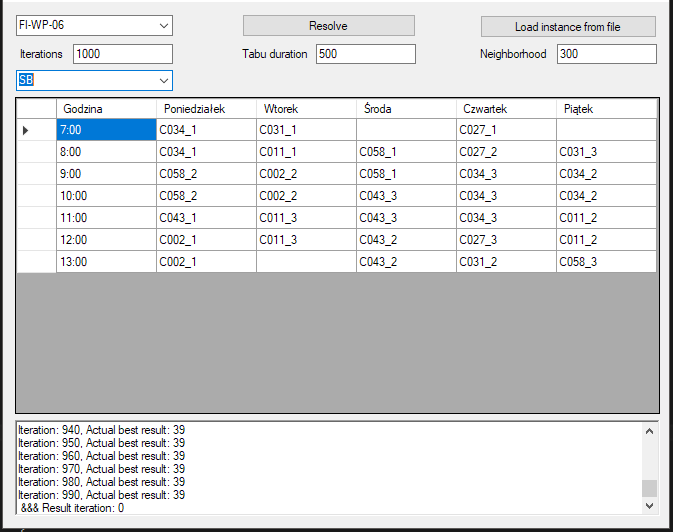
\includegraphics[width=\textwidth] {Aplikacja}
	\caption{Okno główne aplikacji.}
	\label{fig: Aplikacja}
	\end{figure}